\documentclass[paper=a4, fontsize=12pt]{scrartcl} % A4 paper and 11pt font size
\usepackage[margin=1in]{geometry}  

\usepackage[T1]{fontenc} % Use 8-bit encoding that has 256 glyphs
\usepackage{fourier} % Use the Adobe Utopia font for the document - comment this line to return to the LaTeX default
\usepackage[english]{babel} % English language/hyphenation
\usepackage{amsmath,amsfonts,amsthm} % Math packages
\usepackage{enumerate}
\usepackage{graphicx}
\usepackage{caption}

\usepackage{sectsty} % Allows customizing section commands
\allsectionsfont{\raggedright \normalfont\scshape} % Make all sections centered, the default font and small caps

\usepackage{fancyhdr} % Custom headers and footers
\pagestyle{fancyplain} % Makes all pages in the document conform to the custom headers and footers
\fancyhead[R]{\emph{Accelerating flow - Chapter 9}} % No page header - if you want one, create it in the same way as the footers below
\fancyfoot[L]{} % Empty left footer
\fancyfoot[C]{} % Empty center footer
\fancyfoot[R]{\thepage} % Page numbering for right footer
\renewcommand{\headrulewidth}{0pt} % Remove header underlines
\renewcommand{\footrulewidth}{0pt} % Remove footer underlines
\setlength{\headheight}{13.6pt} % Customize the height of the header

\numberwithin{equation}{section} % Number equations within sections (i.e. 1.1, 1.2, 2.1, 2.2 instead of 1, 2, 3, 4)
\numberwithin{figure}{section} % Number figures within sections (i.e. 1.1, 1.2, 2.1, 2.2 instead of 1, 2, 3, 4)
\numberwithin{table}{section} % Number tables within sections (i.e. 1.1, 1.2, 2.1, 2.2 instead of 1, 2, 3, 4)

%----------------------------------------------------------------------------------------
%	TITLE SECTION
%----------------------------------------------------------------------------------------

\newcommand{\horrule}[1]{\rule{\linewidth}{#1}} % Create horizontal rule command with 1 argument of height

\author{\vspace{-5ex}}
\date{\vspace{-10ex}}
\title{	
\normalfont \normalsize 
\textsc{Chem-Eng 321: Fluid Mechanics} \\ [10pt] % Your university, school and/or department name(s)
\horrule{0.5pt} \\[0.2cm] % Thin top horizontal rule
\huge Accelerating Flow \\ (Denn Chapter 9) \\ % The assignment title
\horrule{2pt} \\[0.2cm] % Thick bottom horizontal rule
}


\begin{document}

\maketitle % Print the title

\thispagestyle{empty}

\section*{Learning Objectives}

\begin{enumerate}
\item Derive and analyze detailed microscopic flow model for accelerating flow using Dimensional Analysis and the Similarity Solution
\item Derive and analyze detailed microscopic flow model for accelerating flow using the Integral Approximation method

\end{enumerate}

\section*{Scenario}

Consider an infinite plate with fluid on top:

\vspace{15ex} 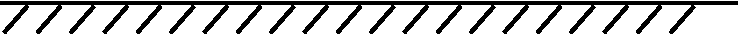
\includegraphics[scale=0.8]{plate.pdf}

\vspace{5ex} We seek a velocity field. 

\section*{Deriving our model}

We know that $v_x(y,t)$, $v_y=0=v_z=0$ just from our intuition and experience from before. (continuity equation satisfied)

We turn to the $x$ component of our Navier-Stokes equations:

\vspace{2ex} \begin{equation*}
\hspace*{-7cm} \rho \frac{\partial v_x}{\partial t} = \eta \frac{\partial^2 v_x}{\partial y^2}
\end{equation*}

Or:

\vspace{2ex} \begin{equation*}
\hspace*{-7cm} \frac{\partial v_x}{\partial t} = \nu \frac{\partial^2 v_x}{\partial y^2}
\end{equation*}

\newpage

\subsection*{Initial Conditions}

\vspace{10ex} \subsection*{Boundary Conditions}


\vspace{15ex} \subsection*{Expected Behavior}


\vspace{15ex}  \begin{figure}[ht]
\centering
\begin{minipage}[b]{0.3\linewidth}
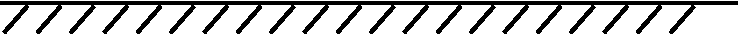
\includegraphics[scale=0.3]{plate.pdf}
\end{minipage}
\quad
\begin{minipage}[b]{0.3\linewidth}
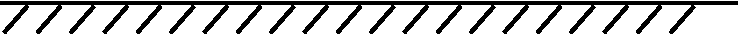
\includegraphics[scale=0.3]{plate.pdf}
\end{minipage}
\quad
\begin{minipage}[b]{0.3\linewidth}
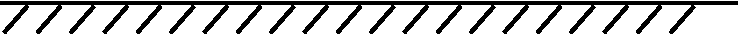
\includegraphics[scale=0.3]{plate.pdf}
\end{minipage}
\end{figure}

\vspace{4ex} How would we solve for $v_x(y,t)$?

\vspace{1ex} \section*{Dimensional Analysis and Similarity Solution Method}



\vspace{2ex}  Define $u(y,t)=v_x(y,t)/U$

\vspace{1ex}  \begin{equation*}
\hspace*{-7cm} \frac{\partial u}{\partial t} = \nu \frac{\partial^2 u}{\partial y^2}
\end{equation*}

\vspace{2ex}  \begin{itemize}
  \item 
  \item 
\end{itemize}

\vspace{4cm} \begin{equation*}
\hspace*{-7cm} u=f(
\end{equation*}

\newpage

Interpreting our dimensionless group we will see that 

\begin{itemize}
  \item $\sqrt{\nu t}$
  \item $\frac{y}{\sqrt{\nu t}}$
\end{itemize}

\subsection*{Similarity Solution}

Velocity profile $u(y,t)$ looks similar at different times when plotted vs the relative distance $\frac{y}{\sqrt{\nu t}}$.

By convention, we use the \underline{similarity variable} ($\zeta$): 

 \begin{equation*}
\hspace*{-7cm} \zeta=\frac{y}{\sqrt{4 \nu t}}
\end{equation*}

\vspace{1cm} We seek a solution to $u(\zeta)$ instead of $u(y,t)$. First we need to rewrite our differential equations and initial/boundary conditions in terms of $\zeta$ using chain rule:

First with respect to time $t$:
  \vspace{0.5cm} \begin{equation*}
\hspace*{-7cm} \frac{\partial u}{\partial t} =\frac{du}{d\zeta} \frac{\partial \zeta}{\partial t}, ~ \hspace*{2cm} \frac{\partial \zeta}{\partial t} = 
\end{equation*}

 \vspace{1cm} \begin{equation*}
\hspace*{-7cm} \Rightarrow \frac{\partial u}{\partial t} =  \Bigg[  \hspace*{3cm}  \Bigg]  \frac{du}{d \zeta} 
\end{equation*}

  \vspace{0.5cm} Next with respect to distance from the plate $y$:

  \vspace{0.5cm}  \begin{equation*}
\hspace*{-7cm} \frac{\partial u}{\partial y} =\frac{du}{d\zeta} \frac{\partial \zeta}{\partial y}, ~ \hspace*{2cm} \frac{\partial \zeta}{\partial y} = 
\end{equation*}

 \vspace{1cm} \begin{equation*}
\hspace*{-7cm} \Rightarrow \frac{\partial u}{\partial y} =  \Bigg[  \hspace*{3cm}  \Bigg] \frac{du}{d \zeta} 
\end{equation*}

  \vspace{0.5cm} Now let's go back to our Navier-Stokes term:


\vspace{0.5cm} \begin{equation*}
\hspace*{-8cm} \frac{\partial^2 u}{\partial y^2} = \frac{\partial}{\partial y} \left(  \frac{\partial u}{\partial y}  \right) = \frac{\partial}{\partial y} \Bigg[  \hspace*{3cm}  \Bigg]  = 
\end{equation*}

 \vspace{1cm} \begin{equation*}
\hspace*{-7cm} \frac{\partial^2 u}{\partial y^2}  =  \hspace*{7cm} =
\end{equation*}

\newpage

Plug back into our Navier-Stokes Equation:

\vspace{1ex}  \begin{equation*}
\hspace*{-7cm} \frac{\partial u}{\partial t} = \nu \frac{\partial^2 u}{\partial y^2}
\end{equation*}

\vspace{1ex}  \begin{equation*}
\hspace*{-2cm} \Bigg[  \hspace*{4cm}  \Bigg] \frac{d u}{d \zeta} = \Bigg[  \hspace*{4cm}  \Bigg]  \frac{d^2 u}{d \zeta^2}
\end{equation*}

\vspace{1ex}  \begin{equation*}
\hspace*{-2cm} \Bigg[  \hspace*{3cm}  \Bigg] \frac{d u}{d \zeta} = \Bigg[  \hspace*{3cm}  \Bigg]  \frac{d^2 u}{d \zeta^2}
\end{equation*}

\vspace{1ex}  \begin{equation*}
\hspace*{-2cm} \frac{d^2 u}{d \zeta^2} = \hspace*{2cm} \frac{d u}{d\zeta} 
\end{equation*}

\vspace{2ex}   Now let's consider the boundary/initial conditions in terms of our similarity variable and relative velocity

\vspace{2ex}  \begin{itemize}
  \item $t=0 \hspace*{0.5cm} \Rightarrow  \hspace*{0.5cm} \zeta = $
  \item $y=0 \hspace*{0.5cm} \Rightarrow \hspace*{0.5cm} \zeta = $
  \item $y=\infty \hspace*{0.5cm} \Rightarrow \hspace*{0.5cm} \zeta = $
\end{itemize}

\vspace{2ex}  At this stage, we have

\vspace{1ex}  \begin{equation*}
\hspace*{-7cm} \frac{d^2 u}{d \zeta^2} = 
\end{equation*}

\vspace{1ex}   Now let's try to solve it. Let $v=\frac{du}{d\zeta}$

\vspace{1ex}  \begin{equation*}
\hspace*{-7cm} \frac{dv}{d\zeta} = 
\end{equation*}

\vspace{1ex}   We can separate variables

\vspace{1ex}  \begin{equation*}
\hspace*{-7cm} \frac{dv}{v} = 
\end{equation*}

\vspace{1ex}   Then integrate

\vspace{1ex}  \begin{equation*}
\hspace*{-7cm} \ln{v}=
\end{equation*}

\vspace{1ex}   And exponentiate

\vspace{1ex}  \begin{equation*}
\hspace*{-7cm} v=
\end{equation*}

\newpage

\vspace{1ex}   Plug back in for $v$:

\vspace{1ex}  \begin{equation*}
\hspace*{-7cm} \frac{du}{d\zeta} =
\end{equation*}

\vspace{1ex}   Separate variables; integrate using $u=1$ at $\zeta=$

\vspace{1ex}  \begin{equation*}
\hspace*{-7cm} \int\limits_1^{u(\zeta)} du =
\end{equation*}

\vspace{1ex}  \begin{equation*}
\hspace*{-7cm} u(\zeta) - 1 =
\end{equation*}

\vspace{1ex}   To determine $C_1$, use our other boundary condition $u(\zeta)=0$ at $\zeta =$

\vspace{1ex}  \begin{equation*}
\hspace*{-3cm} 0 - 1 = \hspace*{4cm} \Rightarrow C_1 =
\end{equation*}


\vspace{1cm}  \begin{equation*}
\hspace*{-8cm} u(\zeta) =
\end{equation*}

\vspace{2ex}   Define the \underline{error function} (tabulated function like sine, cosine, tangent but more exotic)

\vspace{1cm}  \begin{equation*}
\hspace*{-7cm} \text{erf}(\zeta) = 
\end{equation*}

\vspace{0.5cm}  \begin{equation*}
\hspace*{-7cm} u(\zeta) = 
\end{equation*}

\vspace{0.5cm}  \begin{equation*}
\hspace*{-7cm} v_x(y,t) = 
\end{equation*}

\vspace{1.5cm}  \hspace*{2cm}\includegraphics[scale=0.7]{graphlines.pdf}

\newpage

Note that for $\frac{y}{\sqrt{4 \nu t}}$

\vspace{1cm} \underline{Boundary Layer}

\vspace{1cm} Here, the boundary layer thickness, $\delta \approx$

\vspace{3cm} \subsection*{Example Numbers}
Boundary layer thickness after one minute

\vspace{5cm} \subsection*{Example Problem}
A long thin wire is surrounded by a viscous fluid that extends to infinity. At $t=0$, the wire is set in motion along its own axis with velocity = $U$.

\vspace{2cm} 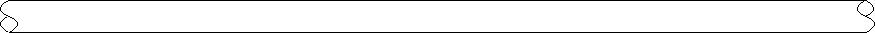
\includegraphics[scale=0.9]{wire.pdf}


\vspace{10ex}  
A. What would we expect the velocity profile to look like over time?
\vspace{15ex}  
\begin{figure}[ht]
\centering
\begin{minipage}[b]{0.3\linewidth}
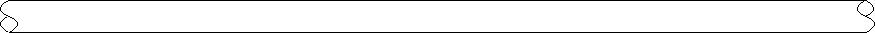
\includegraphics[scale=0.3]{wire.pdf}
\end{minipage}
\quad
\begin{minipage}[b]{0.3\linewidth}
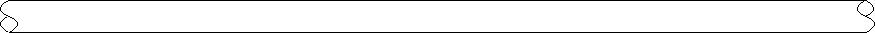
\includegraphics[scale=0.3]{wire.pdf}
\end{minipage}
\quad
\begin{minipage}[b]{0.3\linewidth}
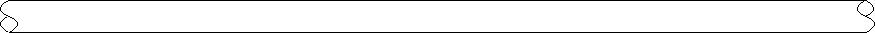
\includegraphics[scale=0.3]{wire.pdf}
\end{minipage}
\end{figure}

\newpage

B. Simplify the Navier-Stokes equations to obtain a partial differential equation governing the time-dependent velocity profile $v_{z}(r,t)$. Also, what are the initial and boundary conditions on the velocity field?

\vspace{0.2cm}  \begin{equation*}
\rho \left( \frac{\partial v_z}{\partial t} + v_r \frac{\partial v_z}{\partial r} + \frac{v_{\theta}}{r} \frac{\partial v_z}{\partial \theta} + v_z  \frac{\partial v_z}{\partial z}  \right) =  -\frac{\partial P}{\partial z} + \rho g_z + \eta \left[   \frac{1}{r} \frac{\partial}{\partial r} \left( r \frac{\partial v_z}{\partial r} \right) +  \frac{1}{r^2}  \frac{\partial^2 v_z}{\partial \theta^2} + \frac{\partial^2 v_z}{\partial z^2}  \right]
\end{equation*}

\vspace{4cm}   C. Introduce the appropriate similarity variable ($\zeta$) that allows this problem to be turned into an ordinary differential equation with appropriate boundary conditions. Rewrite the partial differential equations in terms of this variable. Do not solve.

\vspace{6cm}  \begin{equation*}
\hspace{-12cm}   \frac{\partial \zeta}{\partial t} =
\end{equation*}
\vspace{0.2cm} \begin{equation*}
\hspace{-12cm}  \frac{\partial \zeta}{\partial r} =
\end{equation*}

Re-write the partial derivatives

\newpage
\vspace{0.2cm} \begin{equation*}
\hspace{-12cm}  \frac{\partial u}{\partial t} =
\end{equation*}
\vspace{0.2cm} \begin{equation*}
\hspace{-12cm}  \frac{\partial u}{\partial r} =
\end{equation*}
\vspace{0.2cm} \begin{equation*}
\hspace{-12cm}  \frac{\partial^2 u}{\partial r^2} =
\end{equation*}

\newpage

\section*{Integral Approximation Method}

\subsection*{Introduction}

\vspace{7cm} 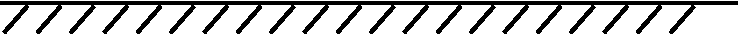
\includegraphics[scale=0.8]{plate.pdf}

\vspace{2ex} Apply momentum conservation to control volume

  \begin{itemize}
  \item Length$=$ 
  \item Width$=$ 
  \item Height$=$ 
\end{itemize}

\vspace{2ex} Rate of Change =

\vspace{0.5cm}  \begin{equation*}
\hspace*{-7cm} \text{momentum in volume} = 
\end{equation*}

\vspace{0.5cm}  \begin{equation*}
\hspace*{-3cm}  = 
\end{equation*}

\vspace{1cm} Do we have to worry about a change in momentum between in surface and out surface?

\vspace{1cm}  \begin{equation*}
\hspace*{-8cm} \text{Rate of change of momentum} = 
\end{equation*}

\vspace{1cm} Forces on the volume?

\newpage

Fluid exerts force on plate =

\vspace{1cm} Plate exerts force on fluid =

\vspace{1cm} Plug in 

\vspace{1cm}  \begin{equation*}
 \hspace*{-5cm} LW \frac{d}{dt} \int_0^{\infty} \rho v_x dy = 
\end{equation*}

\vspace{1cm}  \begin{equation*}
\hspace*{-5cm}  \frac{d}{dt} \int_0^{\infty} \rho v_x dy = 
\end{equation*}

\vspace{1cm} This equation $\Rightarrow$ conservation of 

\vspace{1cm} Whereas, Navier-Stokes equation $\Rightarrow$ conservation of 

\vspace{1cm} Guess approximate velocity profile, $v_x(y)$. We wish to ensure that it satisfies momentum conservation in the 

\vspace{1cm} We assume here that

\begin{itemize}
  \item $v_x=0$ for $y > \delta(t)$
  \item For $y < \delta(t)$, 
\end{itemize}

\vspace{.2cm}  \begin{equation*}
 v_x(y)= U \Phi \left( \frac{y}{\delta} \right)
\end{equation*}

Where $\Phi(0) =$ \hspace*{1cm} and $\Phi(1)=$

\vspace{1cm}  \begin{equation*}
\hspace*{-7cm} \int_0^{\infty} v_x dy = 
\end{equation*}

\vspace{1cm} Let $\xi = \frac{y}{\delta}$ and $dy=\delta d\xi$

\newpage


\vspace{1cm}  \begin{equation*}
\hspace*{-7cm} \int_0^{\infty} v_x dy = 
\end{equation*}

Left-hand side of our momentum balance

\vspace{0.5cm}  \begin{equation*}
 \frac{d}{dt} \int_0^{\infty} \rho v_x dy = \rho \frac{d}{dt}\Bigg[  \hspace*{5cm}  \Bigg] = \Bigg[  \hspace*{5cm}  \Bigg]\frac{d\delta}{dt}
\end{equation*}

Now, the right side

\vspace{0.5cm}  \begin{equation*}
\hspace*{-7cm} -\eta \frac{\partial v_x}{\partial y}  \Bigg|_{y=0} = -\eta U \frac{d}{dy} \Phi \left( \frac{y}{\delta} \right)\Bigg|_{y=0} =
\end{equation*}

\vspace{0.5cm} Plug back into our average momentum balance: 

\vspace{0.5cm}  \begin{equation*}
\hspace*{-7cm} \Bigg[  \hspace*{5cm}  \Bigg]\frac{d\delta}{dt} =
\end{equation*}

\vspace{1cm}  \begin{equation*}
\hspace*{-2cm} \delta \frac{d\delta}{dt} =
\end{equation*}

\vspace{1cm}  \begin{equation*}
\hspace*{-2cm} \frac{1}{2} \frac{d\delta^2}{dt} =
\end{equation*}

\vspace{1cm}  \begin{equation*}
\hspace*{-2cm} \delta^2(t) =
\end{equation*}

\vspace{1.5cm}  \begin{equation*}
\hspace*{-2cm} \delta(t) =
\end{equation*}

\vspace{2cm} We get $\delta \propto$

\newpage

\vspace{0.5cm}  \subsection*{Example 1}

\vspace{0.5cm}  \begin{equation*}
\hspace*{-9cm} \Phi(\xi) = 1 - \xi
\end{equation*}

\vspace{3cm}  \begin{equation*}
\hspace*{-9cm} \delta(t) =
\end{equation*}

\vspace{0.5cm}  \subsection*{Example 2}

\vspace{0.5cm}  \begin{equation*}
\hspace*{-9cm} \Phi(\xi) = 1 - 2\xi + \xi^2
\end{equation*}

\vspace{3cm}  \begin{equation*}
\hspace*{-9cm} \delta(t) =
\end{equation*}

\vspace{0.5cm}  \subsection*{Revisiting the Wire Example}

Consider the same wire problem we looked at earlier with the Similarity Solution set up. In the same way, let's set up; however, since we need to account for viscous force exerted by the wire onto the fluid, let's say that it has a radius of $R$. 

\vspace{3cm}  \includegraphics[scale=0.9]{wire2.pdf}

\newpage

What would be the differential equation to describe the velocity profile in this example?

\vspace{9cm}  If we postulate a shape function to exist, what would our differential equation look like with that included?

\end{document}